\section{\AssertLang -- the assertion language}
\label{sub:SpecO}

Our assertions language, \AssertLang, support ``standard assertions''  as well ``object-capability'' assertions. 
The ``standard assertions''  include implication, quantification etc. In particular, ghost fields may be used to represent user-defined predicates. 
The ``object capability assertions'' express restrictions of an object's eventual authority on some other object.
We define the meaning of ``standard assertions'' in section \ref{sect:semantics:assert:standard}, 
an the meaning of the  ``object-capability'' assertions in  sections \ref{sect:semantics:assert:prtFrom}
and  \ref{sect:semantics:assert:prt}.


\subsection{Syntax of \AssertLang}
The syntax of \AssertLang  is given in Definition \ref{f:chainmail-syntax}.
An assertion may be an expression,   a query of the defining class of
  an object, the usual connectives and quantifiers, along 
with two non-standard assertion forms:
(1) \emph{Internal/external} and (2) \emph{Protection}, inspired by the capabilities literature, and
\footnote{TODO say how these relate with capability lit;  compare with 
 OOPSLA.}


\begin{definition}
\label{def:assert:syntax}
Generalized expressions, $\re$, and assertions, $A$, in
\AssertLang are defined as follows:

\label{f:chainmail-syntax}
 \[
\begin{syntax}
\syntaxElement{\re}{}
		{
		\syntaxline
				{{\alpha}}
				{{x}}
				{\re.f}
				{\re.f({\overline{\re}})}
		\endsyntaxline
		}
\endSyntaxElement
\\
\syntaxElement{A}{}
		{
		\syntaxline
				{{\re}}
				{{\re} : C}
				{\neg A}
				{A\ \wedge\ A}
				{A\ \vee\ A}
				{\all{x:C}{A}}
				{\ex{x:C}{A}}
		\endsyntaxline
		}
 		{
 		\syntaxline
				{\internal{{\re}}}
 				{\external{{\re}}}
				{\protectedFrom{{\re}} {{\re}}} 
				 {\inside {{\re}}} 
		\endsyntaxline
		}
\endSyntaxElement\\
\end{syntax}
\]
In the above, we expect that $f$ stands  for a field or a ghost-field. 
\end{definition}

\noindent
\textbf{NOTES}  Addresses may appear in assertions; this allows  assertions like $\alpha.bal > 700$, but note that universal quantification over addresses  (eg $\forall \alpha:C.[A]$) is not supported; however, we obtain the same effect through quantification over variables (eg  $\forall x:C.[A]$).  
Morewover, the specification does not distinguish between fields and ghostfields. For instance, $a.balance$ may, in some modules (eg when each account object has a field representing it balance), be a field lookup, while in others (e.g. when the balance is defined though an entry in a lookup table),  it may involve executing a ghost function. 
As we discuss below,  our universal quantification goes only over reachable objects i.e. does not consider objects that ould ger collected if we had a garbage collector, while other systems, eg Dafny quantify over allocated addresses.\footnote{example where this distinction would matter/}
% \footnote{{\textbf{NOTE for us} It also allows assertions like $a1.passwd \neq a2.passwd$, whereas in the past we would have written as $\exists x,y.[\ a1.passwd=x \wedge  a2.passwd=y \wedge x\neq y\ ]$.}} \footnote{{TODO compare with oopsla }}

\begin{definition}[Satisfaction 
of Assertions by module and  state] 
\label{def:chainmail-semantics-all}
of Assertions by module and  state] 
\label{def:chainmail-semantics}
We define satisfaction of an assertion $A$ by a % program 
state $\sigma$ with 
 module $M$ by cases on the shape of $A$, in definitions \ref{def:chainmail-semantics}, \ref{def:chainmail-protection-from}, and 
 \ref{def:chainmail-protection}
\end{definition}

TODO: say why we split the def into three defs. 

\subsection{Semantics of \AssertLang -- first part}
\label{sect:semantics:assert:standard}

% An illustration of the concept of reachable appears in the next subsection, in Fig. \ref{fig:Relevant}.
We   use the evaluation relation, $\eval{M}{\sigma}{e}{v}$,
which says that the expression $e$ evaluates
to value $v$ in the context of state $\sigma$ and module $M$.
As expressions in \LangOO may be recursively defined, their evaluation 
need not   % may not necessarily 
 terminate. Nevertheless, the logic of $A$ remains classical because recursion is restricted
to expressions, and not generally to assertions.
\footnote{
The semantics of $\hookrightarrow$ {is} unsurprising 
(see {the appendices %of the full paper 
\cite{necessityFull}).}
We have taken this approach from \citeasnoun{FASE}, which also contains a mechanized Coq proof that assertions are classical \cite{coqFASE}. } %Fig.\ref{f:evaluation}).


\begin{definition}[Satisfaction 
of Assertions -- first part] 
\label{def:chainmail-semantics}
We define satisfaction of an assertion $A$ by a % program 
state $\sigma$ with 
 module $M$ as:
\begin{enumerate}
\item
\label{cExpr}
$\satisfiesA{M}{\sigma}{{\re}}$ \ \ \ iff \ \ \  $\eval{M}{\sigma}{{\re}}{\true}$
\item
\label{cClass}
$\satisfiesA{M}{\sigma}{{{\re}} : C}$ \ \ \ iff \ \ \  $\eval{M}{\sigma}{{\re}}{\alpha}\   \wedge \ \class{\alpha} {\sigma}= C$
\item
$\satisfiesA{M}{\sigma}{\neg A}$ \ \ \ iff \ \ \  ${M},{\sigma}\nvDash{A}$
\item
$\satisfiesA{M}{\sigma}{A_1\ \wedge\ A_2}$ \ \ \ iff \ \ \  $\satisfiesA{M}{\sigma}{A_1} \   \wedge \ \satisfiesA{M}{\sigma}{A_2}$
\item
$\satisfiesA{M}{\sigma}{A_1\ \vee\ A_2}$ \ \ \ iff \ \ \  $\satisfiesA{M}{\sigma}{A_1}\   \vee \ \satisfiesA{M}{\sigma}{A_2}$

\item
\label{quant1}
$\satisfiesA{M}{\sigma}{\all{x:C}{A}}$ \ \ \ iff \ \ \  
 {$\forall \alpha.[\ \GRelevant \alpha \sigma \wedge  \satisfiesA {M}{\sigma} {\alpha:C}  \ \Longrightarrow   \ \satisfiesA{M}{\sigma} {A[x/\alpha]}\ ]$.} 

\item
\label{quant2}
$\satisfiesA{M}{\sigma}{\ex{x:C}{A}}$ \ \ \ iff \ \ \  
 {$\exists \alpha.[\ \GRelevant \alpha \sigma \wedge  \satisfiesA {M}{\sigma} {\alpha:C}  \ \wedge \ \satisfiesA{M}{\sigma} {A[x/\alpha]}\ ]$.} 
\item
\label{cInternal}
$\satisfiesA{M}{\sigma}{\internal{{\re}}}$ \ \ \ iff \ \ \   $\satisfiesA{M}{\sigma}{{{\re}} : C} \ \wedge\ \ C \in M$
\item
\label{cExternal}
$\satisfiesA{M}{\sigma}{\external{{\re}}}$ \ \ \ iff \ \ \   $\satisfiesA{M}{\sigma}{{{\re}} : C} \ \wedge \ C \notin M$
\end{enumerate}
\end{definition}

\textbf{Notes:}  We use the $\Longrightarrow$ symbol in our meta-language to denote implication while $\rightarrow$ is part of Chainmail syntax.
\footnote{{TODO: explain that$x$ is fresh in $\sigma$  means that $x$ is not in the domain of the top frame, nor in the top continuation of $\sigma$.
 Note, the assumption $x$ is fresh in $\sigma$ has to be justified. Barendregt convention? Or say how we rename if $x$ is not free.}}
\footnote{{TODO: say that any assertion $A(e)$ can be understood as a shorthand for $\exists x. [ x=e \wedge A(x)]$. or  $forall x. [ x=e \rightarrow A(x)]$?? For example, the  assertion   ${\internal{e}}$ is a shorthand for $\exists x. [ x=e \wedge {\internal{x}}]$. QUESTION: do we need to talk about $=$ in the assertion language?}}
In most cases, satisfaction of an assertion not only depends on the state $\sigma$, but 
in some cases it also depends on the module: namely execution of expressions (\ref{cExpr}) might need to look up the definition of ghost fields  in $M$, while 
for internal or external provenance (\ref{cInternal} and \ref{cExternal}) we need to know all the classes defined in $M$.

{\textbf{NOTE}  that the term $\re$ may mention ghost fields, but the paths $\alpha.f_1....f_n$ may not. We see that because the latter are interpreted in $\sigma$. That is, $\satisfiesA{M}{\sigma}{{\alpha_o.f_1...f_n}=\alpha}$ is weaker than $\interpret{\sigma}{\alpha_{o}.f_1...f_n}=\alpha$. TODO: write the latter as a lemma}


\subsection{Semantics of Assertions - second part:
protecting an object from another}

As we already discussed in the introduction\footnote{make sure we do discuss there}, in the object capabilities world permission (ie access  \footnote{cite MarkMiller thesis, and our Permission and Authority revisited} to a capability is a necessary precondition to some effect. Motto "authority implies eventual permission".
In our work, we express this as "lack of eventual permission to the relevant capability implies that the given effect will never take place".
For this, we need the concept of "lack of  eventual permission".  

\sdN{
We define this lack of \sdN{eventual} permission as "protected".  
An object $o$ is \emph{protected  from} another, external, object $o'$, if $o'$ can obtain direct access to   $o$ only if 
$o$ is ``introduced'' to some external object (not necessarily $o'$, but external) by some internal object $o''$.  Here we use ``introduce'' in the Mark Miller sense, whereby $o_1$ is is ``introduced'' to $o_2$ by $o_3$, iff either $o_3$ sends to $o_2$ a message containing $o_1$, 
or $o_2$ made a call to $o_3$, and $o_3$ eventually returns  $o_1$ as the result of the call.
} 

%\sdN{The motivation for protection comes from considering eventual executions, but this condition is less practical. Instead, we can obtain sufficient conditions just by observing the heap. In the definition below, we say that $o$ is protected from $o'$ if the last object on any path from $o'$ to $o$ is internal. 
%}

\begin{definition}[Satisfaction 
of Assertions by module and  state continued -- Protected From] 
\label{def:chainmail-protection-from}
\label{sect:semantics:assert:prtFrom}
We continue the definitions in \ref{def:chainmail-semantics}, and define   
\begin{enumerate}
\item
\label{cProtected}
 $\satisfiesA{M}{\sigma}{\protectedFrom{{\alpha}} {{\alpha_{o}}}}$  \ \ \ \ iff  \ \ \ \ 
% \begin{itemize}
 %\item
 $\alpha\neq \alpha_0$,
% \\
 \ \ \ \  and
  \begin{itemize}
 \item
 $\satisfiesA{M} {\sigma} {\internal{\alpha_0}}$
 \\
 or
 \item
$\forall n\in\mathbb{N}. \forall f_1,...f_n.$
% \\
$
[\ \ \interpret{\sigma}{\alpha_{o}.f_1...f_n}=\alpha \ \ \  \Longrightarrow \ \ \ \satisfiesA{M} {\sigma} {\internal{{\interpret{\sigma}{\alpha_{o}.f_1...f_{n-1}}}}}\ \ ]$
\end{itemize}
%\end{itemize}
\item
$\satisfiesA{M}{\sigma}{\protectedFrom{{\re}} {{\re_{o}}}}$  \ \ \ iff \\
  $\exists \alpha, \alpha_{o}. [\  \ \eval{M}{\sigma}{{\re}}{\alpha}\ \wedge \eval{M}{\sigma}{{\re_0}}{\alpha_0} \  \wedge \ 
  \satisfiesA{M}{\sigma}{\protectedFrom{{\alpha}} {{\alpha_{o}}}}
 \ \  ]$
 \end{enumerate}
 \end{definition} 

% \vspace{.5cm}
\footnote{JAMES' comment: If is possible that "we" do not know the complete heap (eg we only know about the green stuff.) how do we know whether an object is protected. The answer is that we do not know that it is protected, but we do know that our code guarnartees poreservation of protectedness.
%Nevertheless, if the objects are "robust" then we can prove that some properties will be preserved. 
}
\footnote{
OLD COMMENTS: ${\inside {\_}}$  is central to thinking about capabilities. For example, the balance of an account whose
  password is  encapsulated/protected?  will not decrease in the next step.
  Often, API implementations contain objects whose capabilities, while  crucial for the implementation, if exposed,
would break the intended guarantees of the API. Such objects need to remain confined - see
such an example in Section \ref{s:examples}. 
}
\footnote{{\textbf{TODO} make the connection with domination}}
\footnote{SD Can we think of a better name than protection? \kjx{encapsulation}\sdN{No, encapsulation not good}}

Figure \ref{fig:ProtectedFrom} illustrates the concept of an object being protected from another object. All the pink objects are external, and the green objects are internal. The left pane shows the objects that are protected from $o_5$\footnote{QUESTION: should we write $5$ or $o_5$?}, the middle pane shows the objects protected from $o_7$, and the right pane shows the objects protected from $o_2$. We highlight the protected objects in yellow. Thus, all objects except $o_6$ are protected from $o_5$;\ all objects expect $o_8$ are protected from $o_7$;\ and all objects except $o_3$, $o_6$, $o_7$, and $o_8$ are protected from $o_2$. 


\begin{figure}[htb]
\begin{tabular}{|c|c|c|}
\hline \\
\resizebox{4.5cm}{!}{
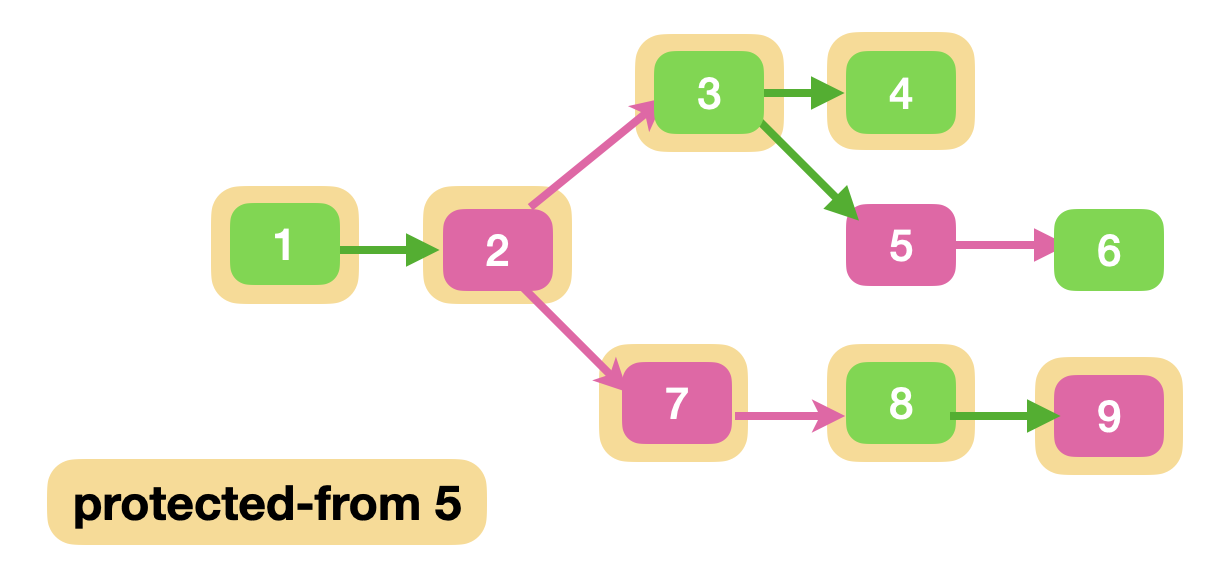
\includegraphics[width=\linewidth]{diagrams/prfA.png}
} 
&
\resizebox{4.5cm}{!}{
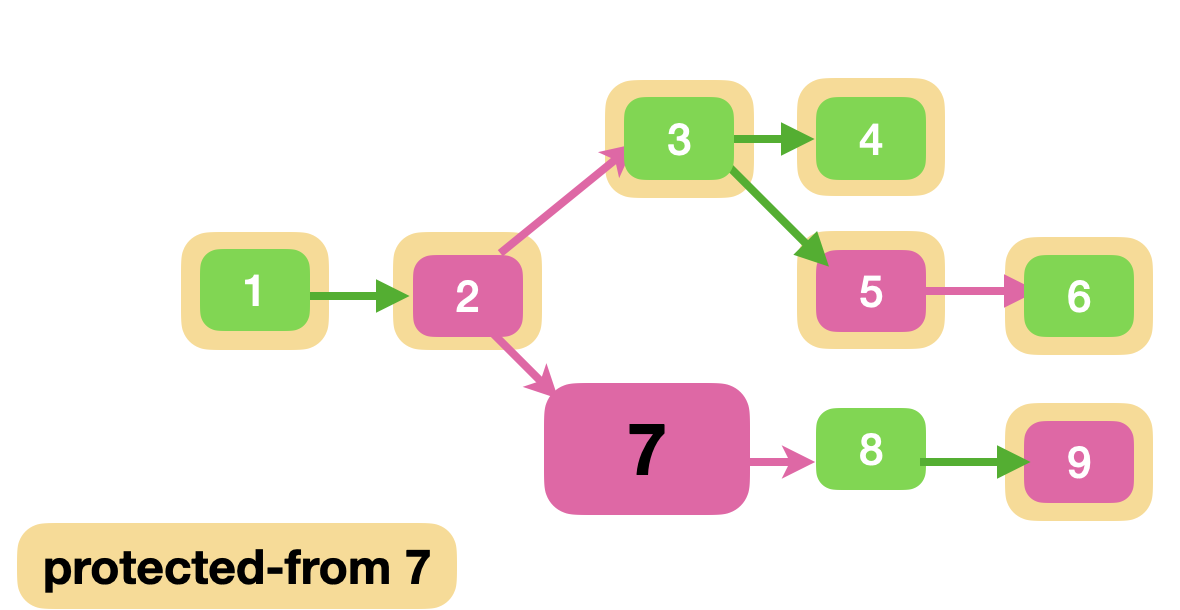
\includegraphics[width=\linewidth]{diagrams/prfB.png}
} 
&
\resizebox{4.5cm}{!}{
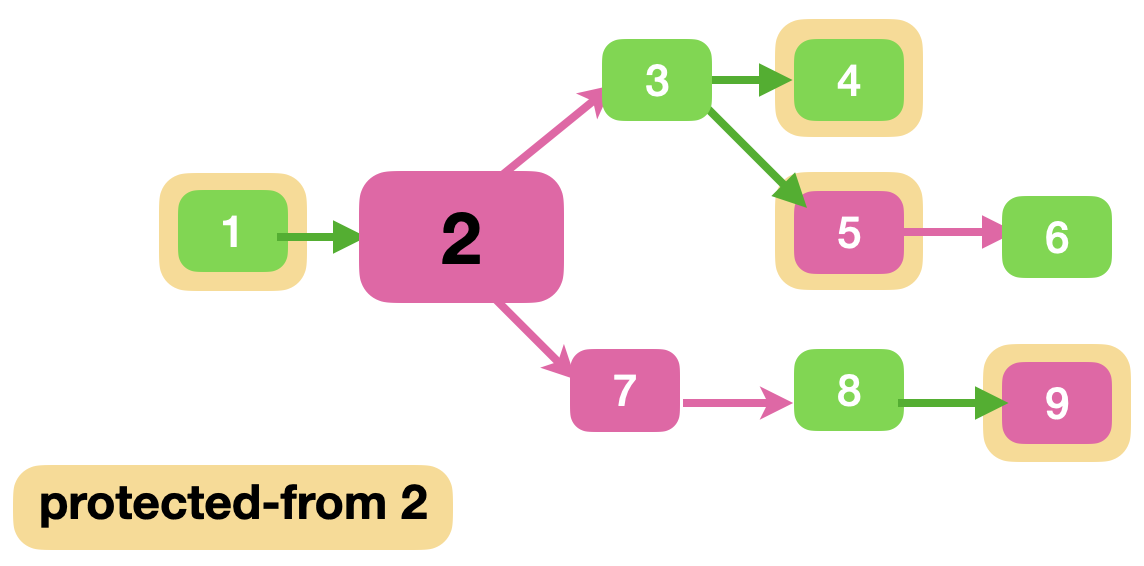
\includegraphics[width=\linewidth]{diagrams/prfC.png}
} 
\\
\hline
protected from $o_5$
&
protected from $o_7$
&
protected from $o_2$
\\
\hline \hline
\end{tabular}
   \caption{Protected From }
   \label{fig:ProtectedFrom}
 \end{figure}
 
 

Note that $o_8$ is not protected from $o_2$ because there is a path from $o_2$ to $0_8$ which only traverses external objects. Note also, that even though $o_9$ is external, it is protected from $o_7$.
Finally, note that $o_6$ is not protected from $o_2$. 
Namely, even through there are some internal objects on the path from $o_2$ to $o_6$, in our current model, these objects are not sufficient to prevent eventual, unmitigated access of $o_2$ to $o_6$: it is possible for $o_2$ to make a call to $o_3$, and then this call to return $o_5$. Once $o_2$ has access to $o_5$, it can also get access to $o_6$. 


\vspace{.1in}

We now introduce the concept of an object being protected.
An object is protected, if it is protected from all locally reachable objects. This could also be understood as 
"an object is protected from the top frame". \footnote{TODO: motivate; many external objects, no matter which one has unprotected access to an object }
 
\begin{definition}[Satisfaction 
of Assertions by module and  state  continued -- Protection] 
\label{def:chainmail-protection}
\label{sect:semantics:assert:prt}
We continue the definitions in \ref{def:chainmail-semantics}, \ref{def:chainmail-protectionFrom } and  define   
\begin{enumerate}
\item
$\satisfiesA{M}{\sigma} {\inside {\re}}$  \ \ \ iff \ \ \ 
\begin{enumerate}
\item
{$\forall \alpha.[ \  \LRelevant {\alpha}  {\sigma}\ \Longrightarrow \ \  \satisfiesA{M}{\sigma}{\protectedFrom{\re} {{\alpha}}}\ ] $}, \ \ \ and 
\item
$\satisfiesA{M}{\sigma}{\external{\prg{this}}}\ \ \Longrightarrow\ \ \forall x\!\in\! \sigma.\ \satisfiesA{M}{\sigma}{x\neq \re}$
\end{enumerate}
\end{enumerate}
\end{definition} 
 
% TODO explain
  Figure \ref{fig:Protected} illustrates the concept of protection. The heap in all three panes is the same as that from  Fig \ref{fig:LReachable}, and 
 ans Fig \ref{fig:ProtectedFrom}. In the left pane the top frame is $\phi_1$; it has  one variable: \prg{this} points to $o_2$. In the middle pane the top frame is $\phi_2$; it has two  variables:   \prg{this} points to $o_3$ and \prg{x} points to $o_7$. In the right pane  the top frame is $\phi_3$; it has two  variables:   \prg{this} points to $o_7$ and \prg{x} points to $o_3$.  

\begin{figure}[htb]
\begin{tabular}{|c|c|c|}
\hline \\
\resizebox{4.5cm}{!}{
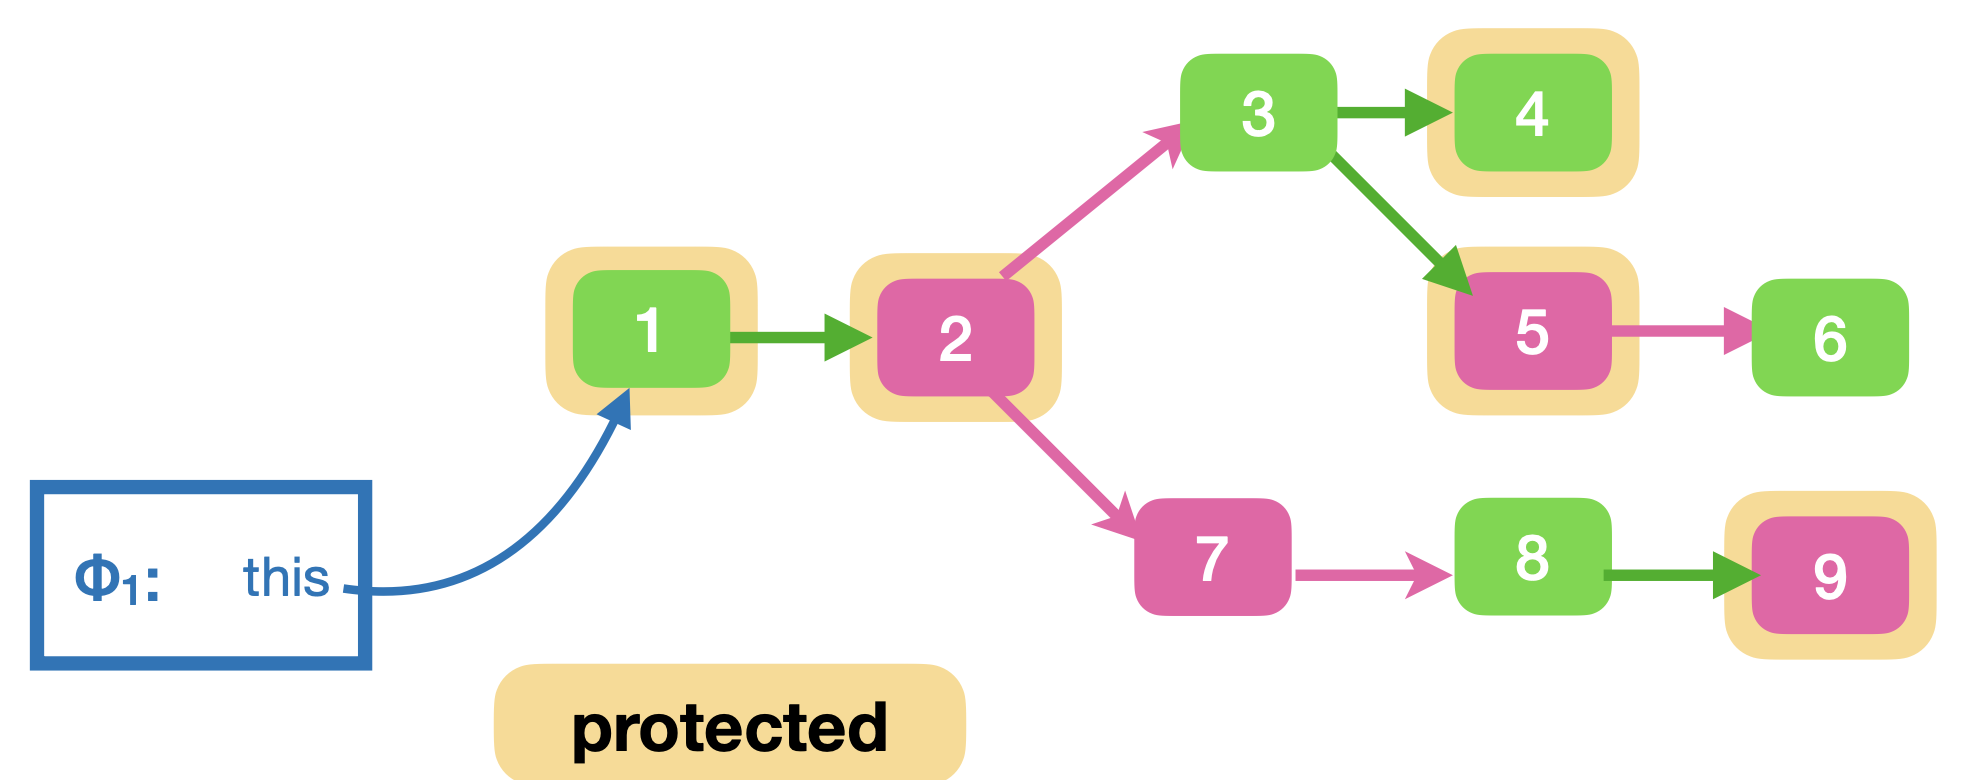
\includegraphics[width=\linewidth]{diagrams/prtFirst.png}
} 
&
\resizebox{4.5cm}{!}{
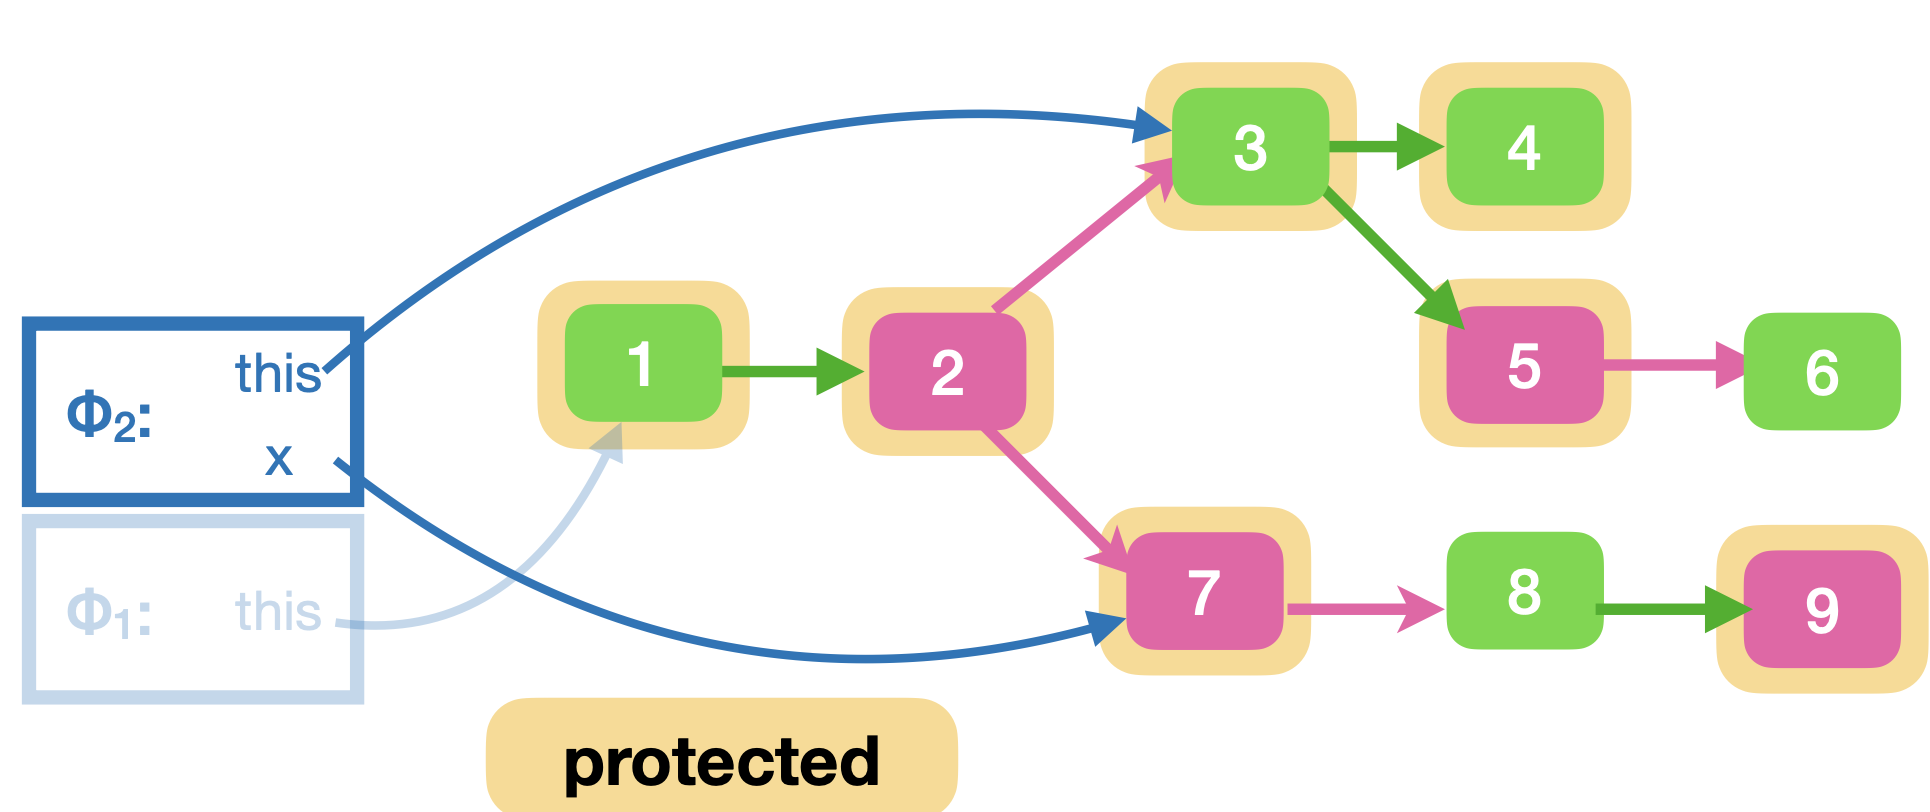
\includegraphics[width=\linewidth]{diagrams/prtSecond.png}
} 
&
\resizebox{4.5cm}{!}{
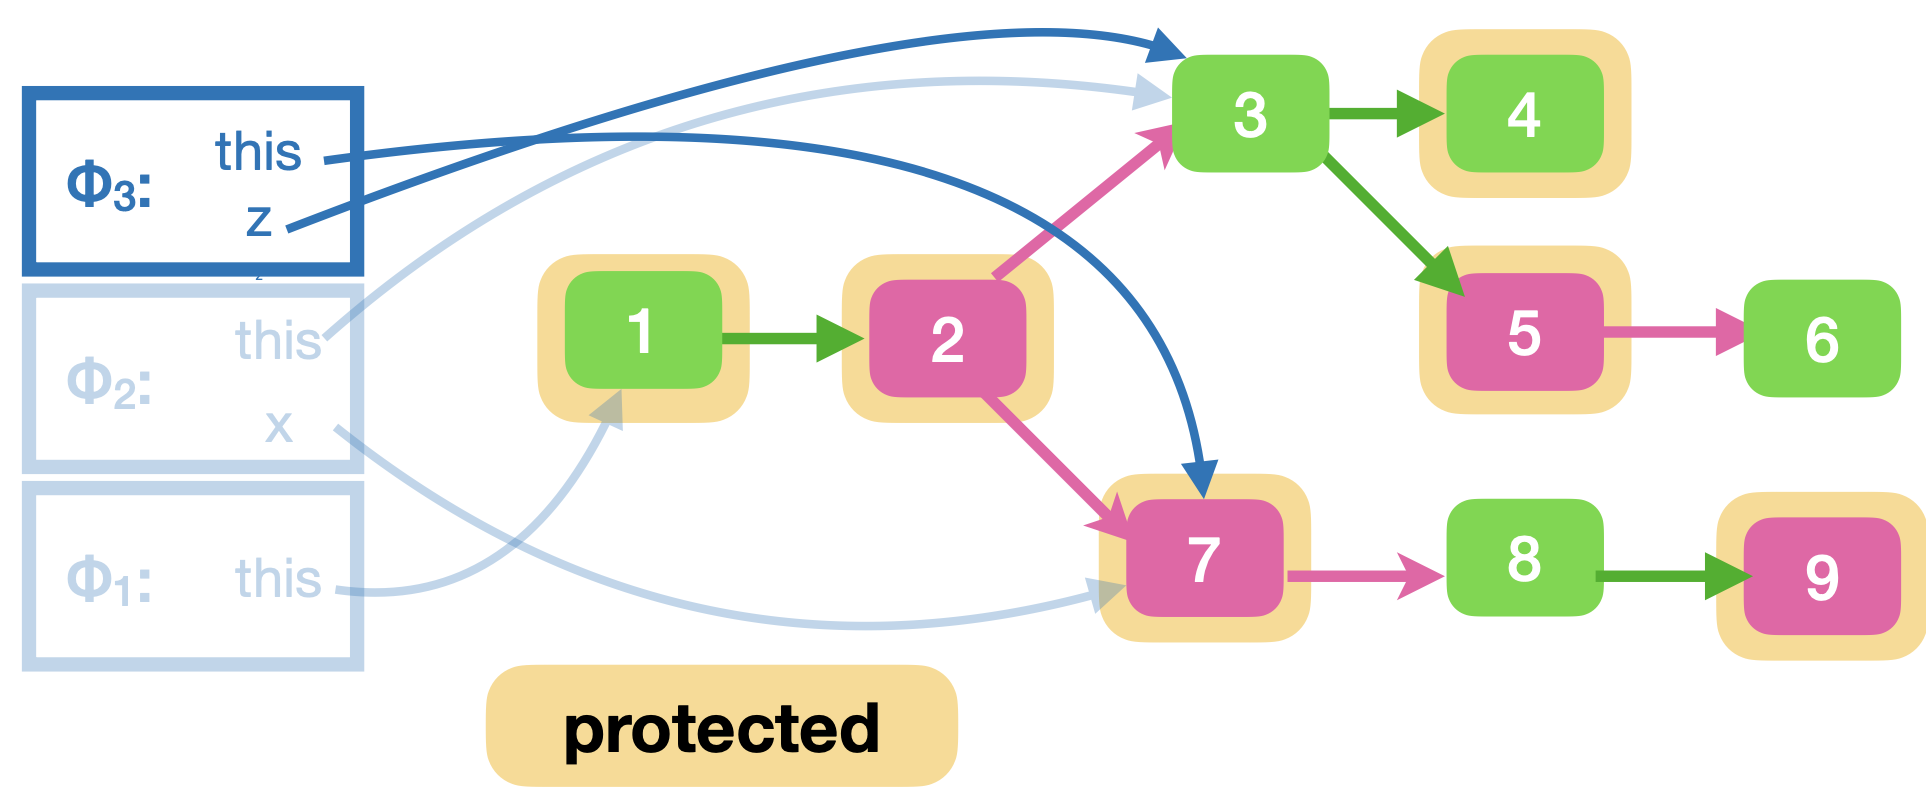
\includegraphics[width=\linewidth]{diagrams/prtLast.png}
} 
\\
\hline
protected  with top frame $\phi_1$ &
protected  with top frame $\phi_2$
&
protected  with top frame $\phi_3$
\\
\hline \hline

\end{tabular}
   \caption{Protected \\
 }
   \label{fig:Protected}
 \end{figure}
 
 
The locally reachable objects from $\phi_1$ were highlighted in the middle pane of.Fig \ref{fig:LReachable}, while the locally reachable object from $phi_2$ as well as from $\phi_3$ were  highlighted in the right pane of that Figure. 
We highlight the protected objects in each pane with a golden hallo.
 Note that $o_3$ is protected from $\phi_2$, but is not protected from $\phi_3$. This is so, because \prg{this} in $\phi_3$ is external, and  $o_3$ is an argument to the call. That means, that during the call, $o_7$ may obtain unmitigated access (permission?) to $o_3$. 
 
 
   
 \subsection{Assertion preservation}
 
\sdN{ In this section we discuss preservation of assertions' satisfaction.
 Lemma \ref{lemma:vars:to:addresses} says that: (1) the validity of an assertion $A$ in the context of a state $\sigma$ is equivalent to the validity of the assertion resulting  from substituting free variables according to the top frame ($A[\sigma]$)}.
(2) if we make a bounded execution step in an external state then relative as well as absolute protection are preserved.
(3) An objects which is protected from  the receiver and arguments of a method call, is protected   after the frame has been pushed onto the stack.

\sdN{
  \begin{lemma}
 \label{lemma:vars:to:addresses}
  For any  module $M$, states $\sigma$, $\sigma'$, assertion $A$,%  addresses $\overline{\apha}:$
  % variables $\overline u$, 
   \atoms $\va$, $\overline \va$, and address $\alpha:$
  % and statement $s$, where   $\sigma'= {\Push {u} {\interpret  {\sigma}{z}} {s} {\sigma} }:$  
  \begin{enumerate}
 \item
$ \satisfiesA {M} {\sigma}  {A}\ \ \ \Longleftrightarrow \ \ \ \  \satisfiesA {M} {\sigma}  {A[\sigma]}$
\item
${
\satisfiesA{M}{\sigma}{\external {\prg{this}} } \ \ \ \wedge \ \ \ \  \leadstoBounded {M}  {\sigma} {\sigma} {\sigma'}}\ \ \ \ \ \ \ \ \   \Longrightarrow$
\begin{itemize}
\item
$ \satisfiesA{M}{\sigma}{\protectedFrom {\alpha} {\va} } \ \ \ \   \Longrightarrow \ \ \ \ \satisfiesA{M}{\sigma'}{\protectedFrom {\alpha} {\va} } $
\item
$ \satisfiesA {M} {\sigma} {\inside {\alpha}}   \ \ \ \   \Longrightarrow \ \ \ \satisfiesA {M} {\sigma'} {\inside {\alpha}} $
\end{itemize}
\item
If $\sigma'\!\in\! {\Pushes   {\interpret  {\sigma}{\va}} {\sigma} }$, then 
\begin{itemize}
\item
 $ \satisfiesA {M} {\sigma'} {\inside {\alpha}}$  
  \\
  $ \Longleftrightarrow$ 
  \item
   $\forall i\in 0..n.[\ \ \satisfiesA{M}{\sigma}{\protectedFrom {\alpha} {\va_i} }  \ \ \wedge\ \ 
 [ \  \satisfiesA{M}{\sigma}{\external {\va_o}} \ \Longrightarrow\   \satisfiesA{M}{\sigma} {\va_i \neq {\alpha}}\ ] \ \  ] $
\end{itemize}
 \end{enumerate}
\end{lemma}
}
 
 
\paragraph{We will prove this later}
Let us use the notation $A \Rightarrow_{\overline z} A'$ for lifting. Then, we want to have

\sdN{
  \begin{lemma}
 \label{lemma:lifts}
  For any  module $M$, states $\sigma$, $\sigma'$, assertion $A$,%  addresses $\overline{\apha}:$
  variables $\overline z:$
\begin{itemize}
\item
  $ \satisfiesA {M} {\sigma}  {A}\ \ \ \wedge \ \ A \Rightarrow_{\overline z} A' \ \ \wedge \ \  \sigma'\in \Pushes {\interpret {\sigma} {z}} {\sigma}$
  \ \ \ \ \ 
% \\
$\Longrightarrow$
\ \ \ \ \ 
% \item
$  \satisfiesA {M} {\sigma'}  {A'[\sigma]}$
\end{itemize}
\end{lemma}
}
 % rests?
 % $ \satisfiesA {M} {\sigma {\inside {\alpha}} \ \ \wedge \ \  {\leadstoBounded {M}  {\sigma} {\sigma} {\sigma'}}\ \ 
%\satisfiesA{M}{\sigma}{\external {\prg{this}} \ \ \ \   \Longleftrightarrow \ \ \ \  \satisfiesA {M} {\sigma' {\inside {\alpha}} $
%\item
%
%
%\Longrightarrow\ \  \satisfiesA {M} {\sigma'} {\inside {\alpha}}$
%\item
%$ \satisfiesA {M} {\sigma {\inside {\alpha}} \ \ \Longrightarrow\ \  \satisfiesA {M} {\sigma'} {\inside {\alpha}}$

 
 \subsection{Discussion of the semantics of assertions}
 
 {Both existential and universal quantification (defined in \ref{quant1} and \ref{quant2}) is done over all objects which are transitively 
accessible any frame in the stack (as in OOPSLA). But note that $\satisfiesA{M}{\sigma} {\inside {y}}$ only considers objects that are locally reachable ..

We do not include quantification over primitive types such as integers as \LangOO is too simple. The 
Coq mechanisation does include primitive types.}
\footnote{TODO: Do we prove the implications as in TACAS, or just rely on TACAS? -- perhaps the former, since we have some new primitives? hmhh}

\subsubsection{Alternative Definition of Protection}

We could have given a weaker definition of protection, which would require that $o$ is protected from $o'$ if $o'$ can obtain direct access to $o$ only if some internal object executes a method. 
The projection of this weaker definition into the heap structure is as below


$\satisfiesA{M}{\sigma}{ {\alpha\ }\textbf{weakPrtFrom}\ {\alpha_o} }$  \ \ \ iff \\
\begin{itemize}
\item $\satisfiesA{M}{\sigma}{\internal{\alpha_0}}$, \\ or
\item 
$\forall n\in\mathbb{N}. \forall f_1,...f_n.$\\
$
[\ \ \interpret{\sigma}{\alpha_{o}.f_1...f_n}=\alpha \ \ \  \Longrightarrow \ \ \ \exists k<n. \satisfiesA{M} {\sigma} {\internal{{\interpret{\sigma}{\alpha_{o}.f_1...f_{k}}}}}\ \ ]$
\end{itemize}


With this, weaker, definition, in Fig. \ref{fig:ProtectedFrom}, object $6$ would be weakly-protected from $2$. Namely,  here 
for $2$  to get access to $6$ it suffices for $3$ to introduce $5$ to $2$, and does not require that some internal object introduces $6$ to some external object\footnote{TODO? Hmhh This would have been clearer if there was also a field pointing from 3 to 5}.

Note however that this alternative definition does not satisfy Lemma \ref{lemma:rel:abs:prot}. For a counterexample,   consider pushing onto the frame $\phi_1$ from Fig. \ref{fig:ProtectedFrom}, a frame $\phi_4$ where $\phi_4(\prg{this})$=$2$. Then, Lemma
\ref{lemma:rel:abs:prot} would promise that $6$ is protected from that frame, even though it is not.




